% ========================================= TEMPLATE INFO =========================================
%
% Author:       Rin-Ha-n
% Version:      1.0
% Last updated: 2025-05-20
% Brief:        A cheatSheet for the module DigDes (Digital Design) at OST FS25

% ================================================================================================
\documentclass[a4paper,landscape,8pt]{extarticle}
% Font size:    8pt
% Paper size:   A4
% style:        twoside (needed, so odd and even pages have different margins)
% orientation:  portrait. (use 'landscape' for landscape orientation)



% ========================================= DOCUMENT INFO =========================================
\def\title{CheatSheet Digital Design}   	     		% title
\def\shorttitle{DigDes}                              	% short title (displayed as PDF title)
\def\dozent{Prof. Dr. Paul Zbinden}                     % lecturer
\def\semester{Fs 2025}								    % semester
\def\author{Ricca Aaron}                           	    % author(s)
\def\repo{https://github.com/Rin-Ha-n/DigDes}       	% repository link
\def\version{1.0\today}                              	% version
\def\pagelimit{4}                                   	% page limit -> causes pages after limit to be red
\def\titleoption{ultra compact}                         % options: ultra compact, compact, normal
\def\enableToC{false}                                   % enable table of contents (true/false)        

\def\sectioncolor{green}                                % section color   (Used green because as shown in psycology studies it calms you) 
\def\subsectioncolor{green}                             % subsection color
\def\subsubsectioncolor{green}                          % subsubsection color

% ================================= PACKAGES, SETUP AND COMMANDS ==================================
% ================================================================================================
%                                   PREAMBLE FOR CHEATSHEET
% ================================================================================================
% This file sets up all packages and commands needed for the cheatsheet template.
% Only essential packages and the title block command are included.
% ================================================================================================

% --------------------------------- ONLY FOR TESTING ----------------------------------------------
\usepackage{lipsum} % For generating dummy text

% --------------------------------- School required package -------------------------------------------
\usepackage{oststud} % Package from the OST school
\usepackage{xcolor} % Color package needed for the oststud package

% --------------------------------- ENCODING AND FONTS -------------------------------------------
\usepackage[T1]{fontenc}         % T1 font encoding for better output
\usepackage{times}               % Times font for main text
\usepackage{inconsolata}         % Inconsolata font for monospaced text
\usepackage[main=english]{babel} % English language/hyphenation

% --------------------------------- PAGE LAYOUT --------------------------------------------------
\usepackage{multicol}            % Support for multi-column layouts
\setlength{\columnseprule}{0.4pt} % Thickness of the vertical line between columns
\usepackage{geometry}            % Flexible page geometry
\geometry{left=3mm, right=3mm, top=3mm, bottom=6mm} % Custom margins

% --------------------------------- MATH & SYMBOLS -----------------------------------------------
\usepackage{amsmath, amssymb, mathtools, bm} % Math packages

% --------------------------------- GRAPHICS & COLORS --------------------------------------------
\usepackage{graphicx}            % Include images
\usepackage{scalerel}            % Scale symbols relative to text
\usepackage{tikz}                % Drawing and diagrams

% Prevent section titles from breaking columns
\usepackage{titlesec}
\titleformat{\section}{\large\bfseries}{\thesection}{1em}{}
\titleformat{\subsection}{\normalsize\bfseries}{\thesubsection}{1em}{}


% --------------------------------- LINKS & QR CODES ---------------------------------------------
\usepackage{hyperref}            % Hyperlinks in PDF
\usepackage{qrcode}              % Generate QR codes

% --------------------------------- CODE LISTINGS ------------------------------------------------
\usepackage{listings}            % Code formatting

% Prevent section and subsection titles from breaking columns in multicols
\usepackage{etoolbox}
\makeatletter
\patchcmd{\section}{\if@col@number \ifnum \col@number >\@ne \columnbreak\fi\fi}{}{}{}
\patchcmd{\subsection}{\if@col@number \ifnum \col@number >\@ne \columnbreak\fi\fi}{}{}{}
\patchcmd{\subsubsection}{\if@col@number \ifnum \col@number >\@ne \columnbreak\fi\fi}{}{}{}
\makeatother

% --------------------------------- TITLE BLOCK COMMAND ------------------------------------------
% This command creates the title block with QR code, version, title, semester, lecturer, authors, and repo link.
\newcommand{\cheatsheettitle}{%
    \begin{minipage}[t]{0.2\columnwidth}
        \vspace{-0.225\columnwidth}
        \qrcode[level=L, version=0, height=0.9\columnwidth]{\repo}\\[1mm]
        \normalfont\footnotesize V \version{} \hspace{1em}
        \smallskip
    \end{minipage}\hfill
    \begin{minipage}[t]{0.79\columnwidth}
        \raggedright%
        \normalfont\Huge\bfseries\title{}\\[1mm]
        \normalfont\Large\semester\ --\ \dozent{}\\
        \large Autoren:\ \author{}\\[1mm]
        \normalsize\url{\repo}
    \end{minipage}
}

% --------------------------------------- DOCUMENT SETTINGS ---------------------------------------
\hypersetup{hidelinks,
% set pdf metadata
            pdfauthor={\author},
            pdftitle={\shorttitle},
            pdfsubject={\title\ \semester},
            pdfkeywords={Gahn go lerne!!}}

% set style for URLs
\urlstyle{same} % sets url font to the same as the preceeding text

% set page layout
\geometry{left=3mm, 
          right=3mm, 
          top=3mm, 
          bottom=6mm, 
          headheight=0mm, 
          headsep=0mm, 
          footskip=4mm,
        %   showframe,
          }

\setlength{\columnsep}{1.5mm}       % distance between columns
\setlength{\columnseprule}{0.1pt}   % thickness of column separation line
\setlength{\parindent}{0pt}         % no paragraph indentation

\setcounter{tocdepth}{2}            % only display sections and subsections in toc


% --------------------------------- SECTION HEADER COLORS -----------------------------------------------
\newcommand{\coloredsection}[1]{%
  \colorbox{\sectioncolor!60}{\parbox{\dimexpr\linewidth-2\fboxsep}{\thesection\ #1}}}

\newcommand{\coloredsubsection}[1]{%
  \colorbox{\subsectioncolor!40}{\parbox{\dimexpr\linewidth-2\fboxsep}{\thesubsection\ #1}}}

\newcommand{\coloredsubsubsection}[1]{%
  \colorbox{\subsubsectioncolor!20}{\parbox{\dimexpr\linewidth-2\fboxsep}{\thesubsubsection\ #1}}}

\titleformat{\section}
  {\normalfont\Large\bfseries}
  {}
  {0pt}
  {\coloredsection}

\titleformat{\subsection}
  {\normalfont\large\bfseries}
  {}
  {0pt}
  {\coloredsubsection}

\titleformat{\subsubsection}
  {\normalfont\normalsize\bfseries}
  {}
  {0pt}
  {\coloredsubsubsection}


% ================================================================================================
%                                   END OF PREAMBLE
% ================================================================================================ % Used to include minimum required packages and settings

% ---------------------------------- Code Block word Color ----------------------------------------------
\lstdefinelanguage{VHDL}{
  morekeywords={architecture,begin,block,case,component,configuration,else,elsif,end,entity,for,function,generate,if,is,loop,package,port,process,return,signal,then,type,use,variable,wait,when,while,with,library,assert,report,after,until,others,all,constant,procedure,of,downto,to,in,out,inout,buffer,linkage,guarded,open,range,record,select,transport,reject,units,group,file,access,shared,new,next,null,exit,abs,not,and,or,xor,nand,nor,sll,srl,sla,sra,rol,ror},
  sensitive=true,
  morecomment=[l]--,
  morestring=[b]",
  morestring=[b]',
  morekeywords=[2]{bit,bits,bit_vector,std_logic,std_logic_vector,integer,natural,signed,unsigned}
}
\lstset{
  basicstyle=\ttfamily\footnotesize,
  keywordstyle=\color{violet}\bfseries,
  keywordstyle=[2]\color{yellow!80!black}\bfseries,
  commentstyle=\color{OSTDarkGreen}\itshape,
  stringstyle=\color{orange},
  numbers=left,
  numberstyle=\tiny\color{gray},
  stepnumber=1,
  xleftmargin=1.5em,       % small margin to keep numbers inside column
  framexleftmargin=0pt,  % no extra frame margin
  breaklines=true,
  showstringspaces=false,
  tabsize=2,
  aboveskip=0pt,
  belowskip=0pt,
  columns=flexible       % <--- THIS IS IMPORTANT!
}

% ---------------------------------- Code Block lines number Color ----------------------------------------------
\usepackage{xparse}
\usepackage{xstring}
\usepackage{etoolbox}
\makeatletter
\NewDocumentCommand{\highlightlines}{mmm}{%
  \StrCut{#1}{,}{\FirstLine}{\RestLines}%
  \def\@tempa{#1}%
  \edef\@tempb{\number\value{lstnumber}}%
  \def\found{0}%
  \renewcommand{\do}[1]{%
    \ifnum\pdfstrcmp{\@tempb}{##1}=0
      \def\found{1}%
    \fi
  }%
  \docsvlist{#1}%
  \ifnum\found=1
    \begingroup
      \setlength{\fboxsep}{0pt}%
      \colorbox{#2}{\strut #3}%
    \endgroup
  \else
    #3%
  \fi
}
\makeatother

% =========================================== DOCUMENT ============================================
\begin{document}
    \begin{multicols}{3}
        \raggedcolumns
        \cheatsheettitle
        \section{Introduzione}

% ==================== COMPONENT CHOICE ========================
    \subsection{Scelta/caratteristiche dei componenti}
        \noindent
        \begin{minipage}[t]{0.48\columnwidth}
            \vspace{0pt}  %<-- ensures top alignment
            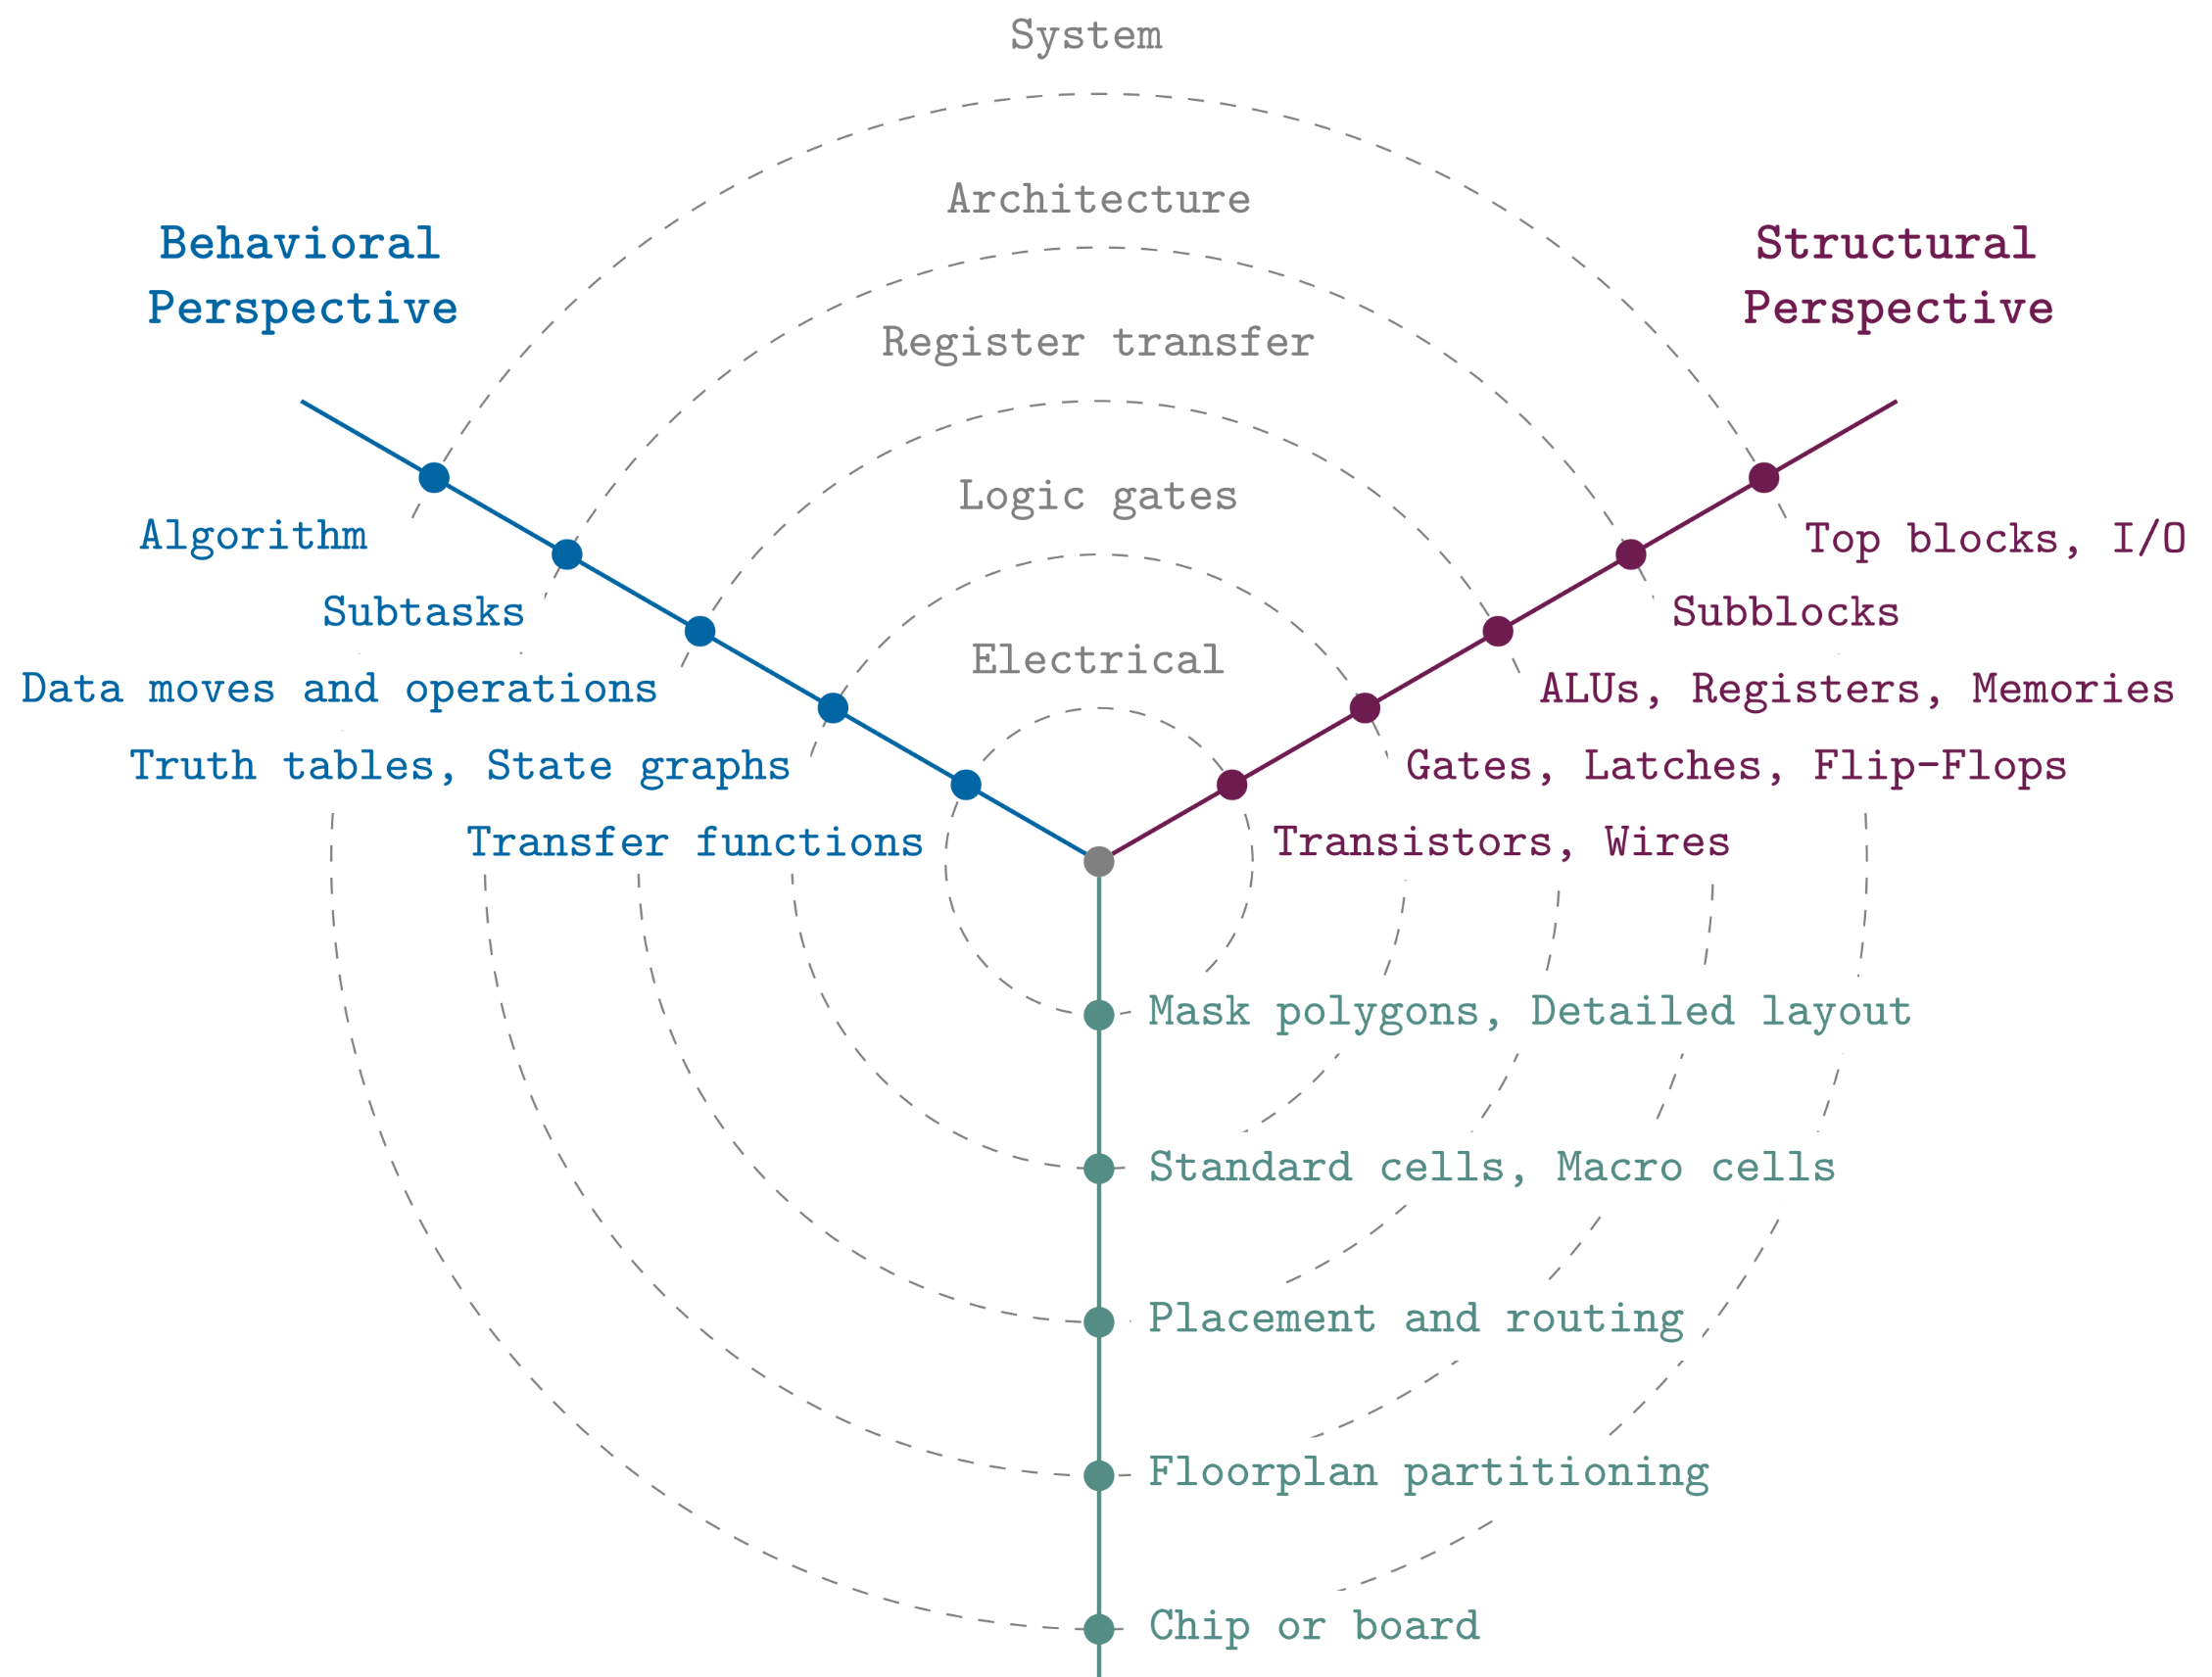
\includegraphics[width=\linewidth]{Images/DevelopmentModel.png}
        \end{minipage}
        \hfill
        \begin{minipage}[t]{0.48\columnwidth}
            \vspace{0pt}  %<-- ensures top alignment
            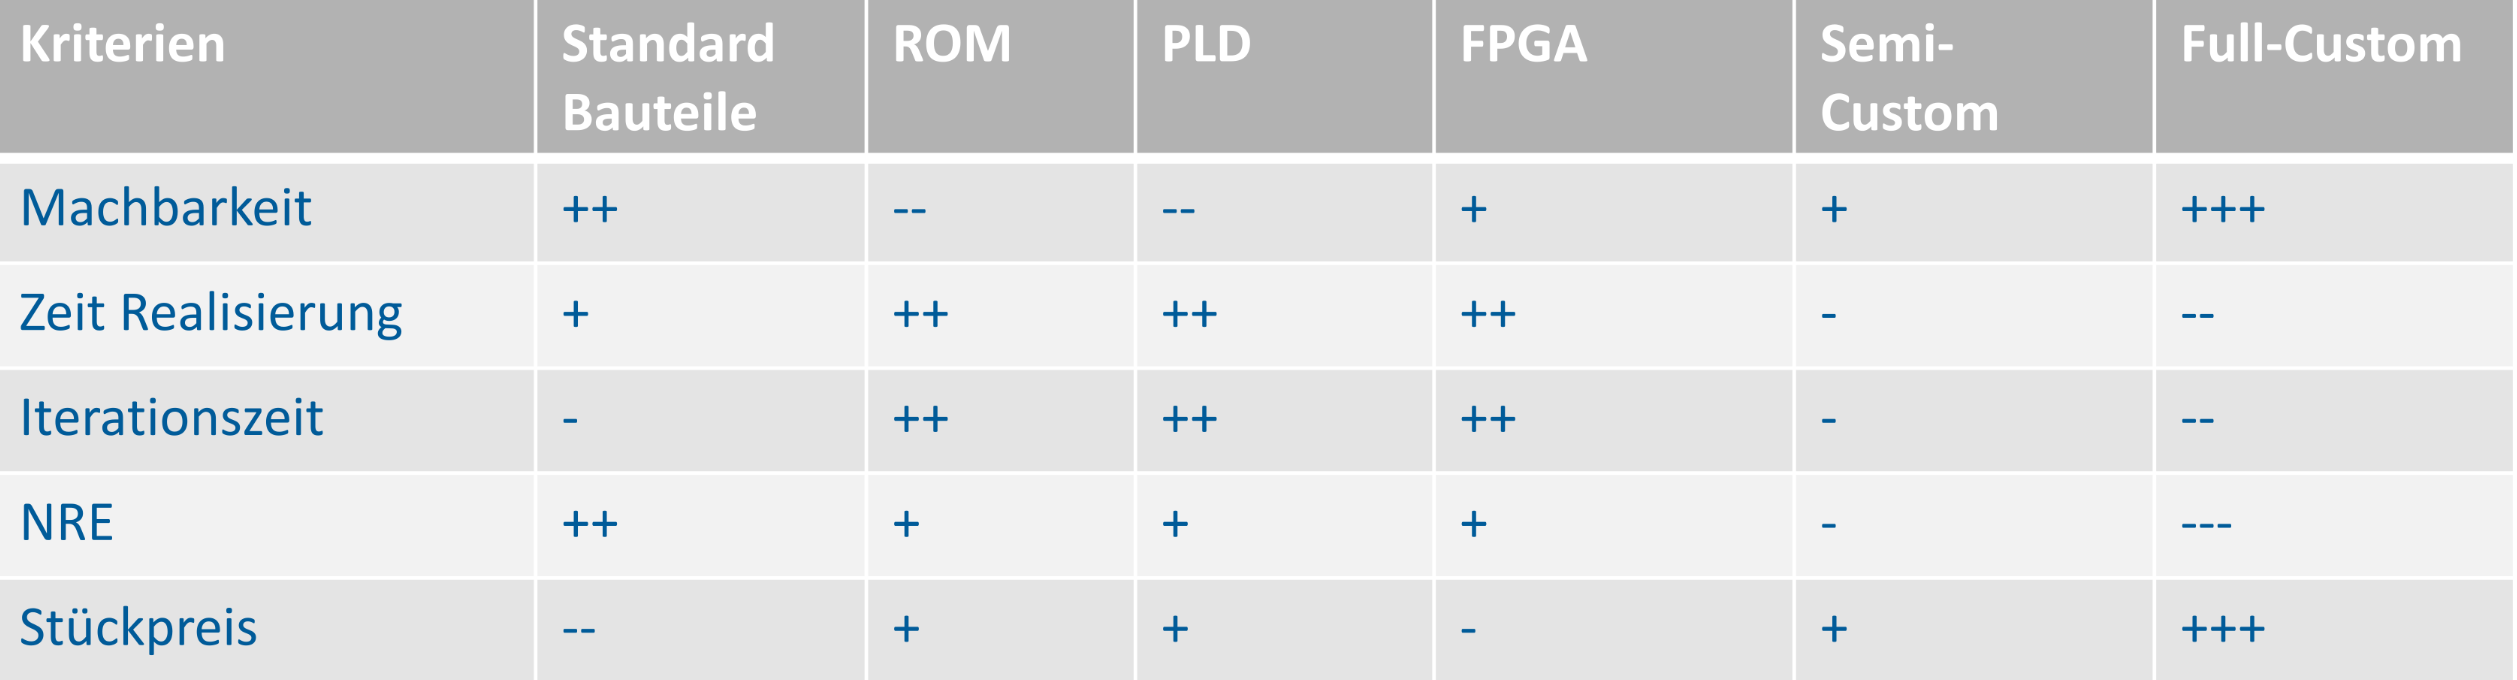
\includegraphics[width=\linewidth]{Images/WhalDerRealisirungsform.png}\\[1ex]
            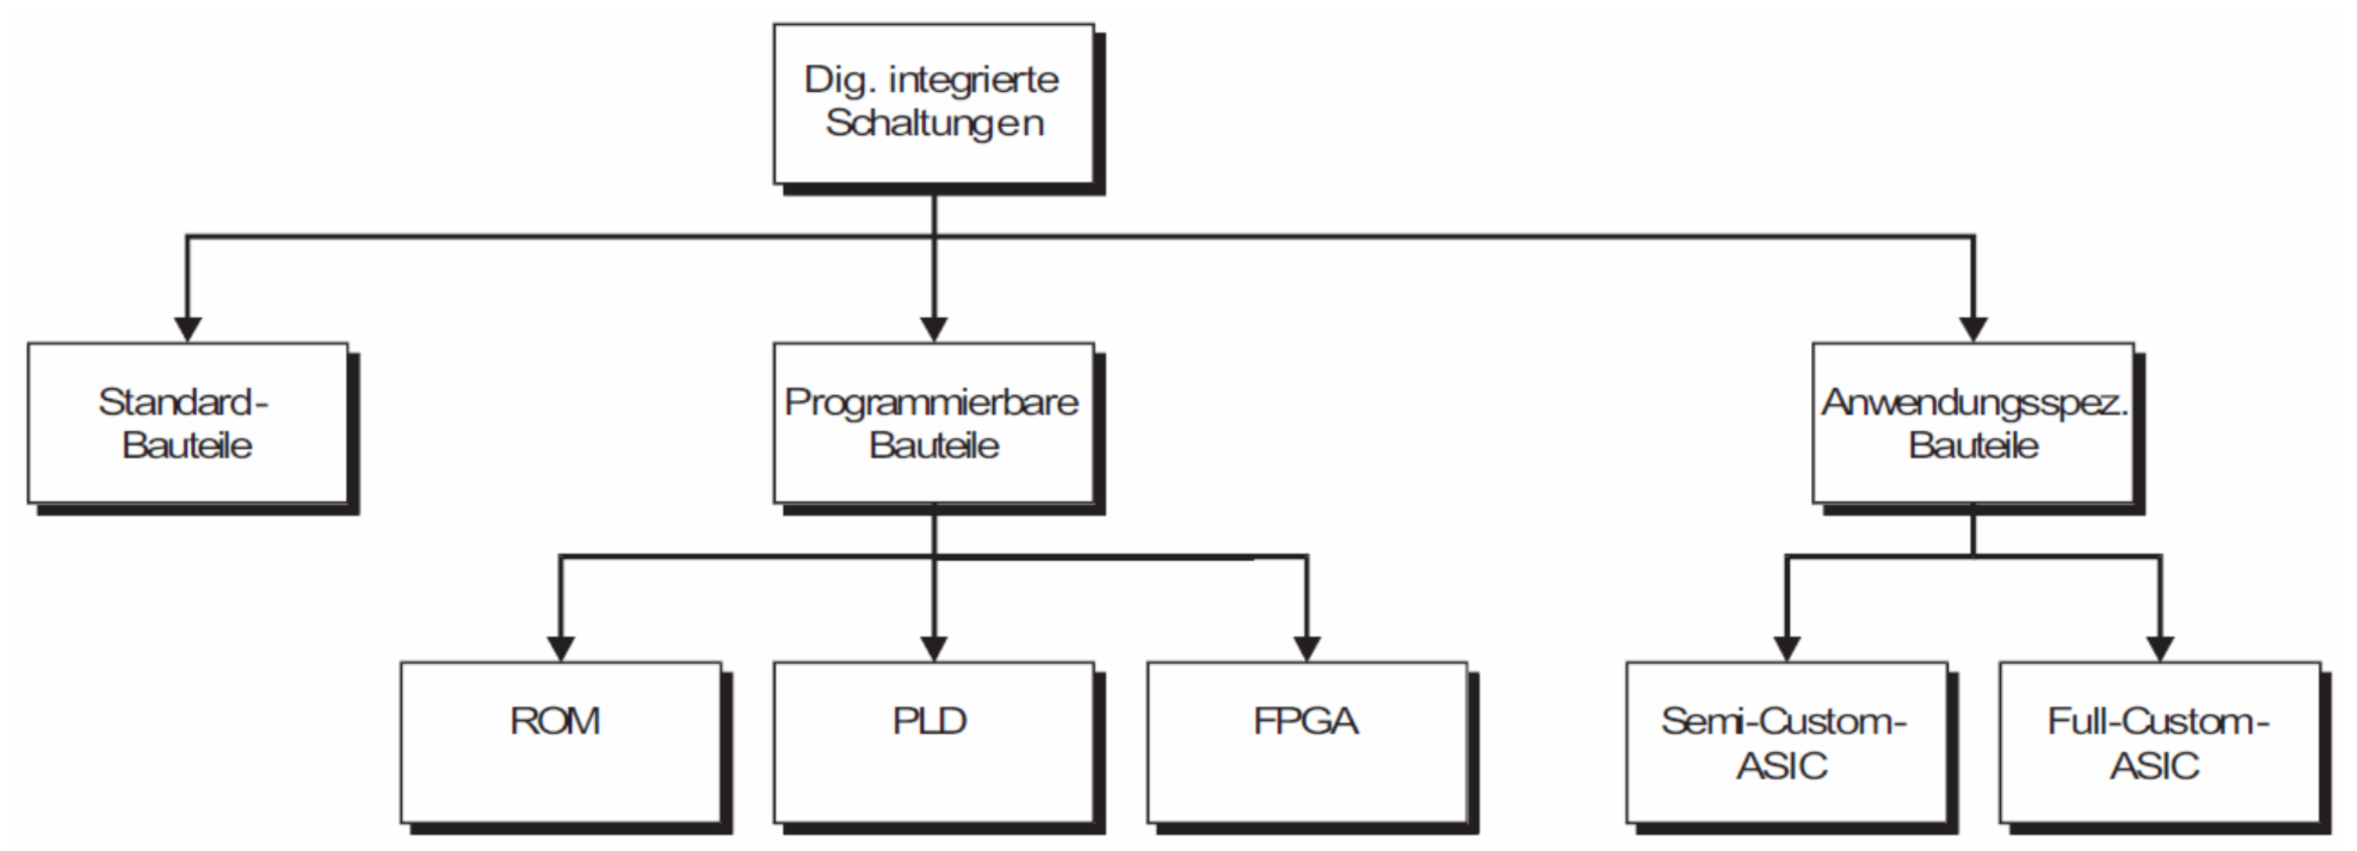
\includegraphics[width=\linewidth]{Images/ClassificationeDeiComponenti.png}
        \end{minipage}


% ==================== DESGIN MUSTER ========================
    \subsection{Guida al design}
        \begin{minipage}[t]{0.48\columnwidth}
            \vspace{0pt} % ensures top alignment
            \begin{enumerate}
                \item Design / Entry
                \item Funktionale Simulation
                \item Synthese
                \item Implementierung
                \begin{itemize}
                    \item Logikoptimierung
                    \item Platzierung
                    \item Verdrahtung
                \end{itemize}
                \item Timing Simulation
                \item Statische Timing Analyse
                \item Herstellungsdatenerzeugen
            \end{enumerate}
        \end{minipage}
        \hfill
        \begin{minipage}[t]{0.48\columnwidth}
            \vspace{0pt} % ensures top alignment
            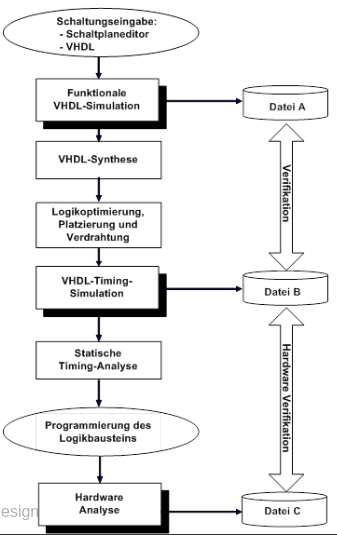
\includegraphics[width=\linewidth]{Images/GuidaDesign.png}
        \end{minipage}


% ==================== BUBBLE DIAGRAM ========================
    \subsection{Bubble diagram}
        \begin{minipage} [t]{0.48\columnwidth}
            \vspace{0pt} % ensures top alignment
            \begin{itemize}
                \item \textbf{Bolle}: Ogni bolla rappresenta uno stato
                \item \textbf{Freccie}: Condizione per passare da uno stato all'altro dev'essere scritta accanto alla freccia.
                \item \textbf{Moore}: Gli output sono associati agli stati, quindi scritti dentro a quest'ultimi.
                \item \textbf{Melay}: Gli output sono associati alle transizioni, quindi scritti accanto alle frecce.
            \end{itemize}
        \end{minipage}
        \begin{minipage} [t]{0.48\columnwidth}
            \vspace{0pt} % ensures top alignment
            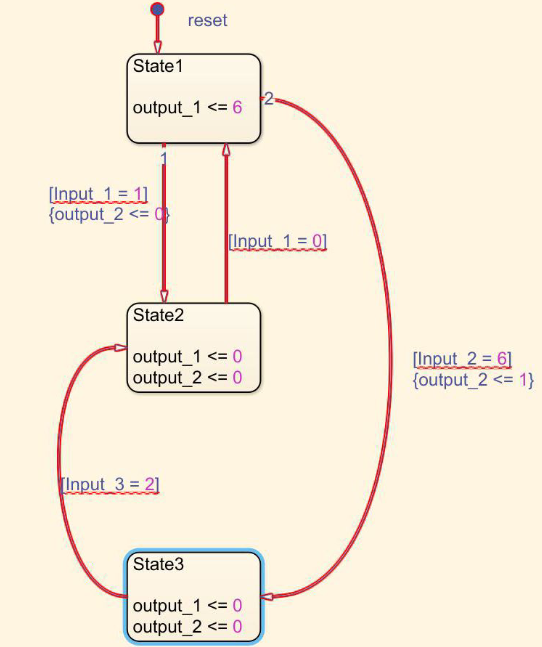
\includegraphics[width=\linewidth]{Images/BubbleDiagram.png}
        \end{minipage}
        \section{Programmazione VHDL}
% =========================================== LIBRARY =========================================
    \subsection{Library}
        Una libreria puo contenere componenti e o pachetti. I componenti sono descrizione di circuiti e realizzazione specifiche,
        vengono memorizzati nella libreria in modo da poter essere riutilizati piu volte e da piu progettisti contemporaneamente.\\
        I blocchi di codice di una libreria sono memorizzati in forma compilata, direttamente eseguibile.\\
        Contenuto di una libreria: Components, Packages, Functions, Procedures, Declarations.
        \begin{lstlisting}[language=VHDL]
library ieee; 
use ieee.std_logic_1164.all; -- CPP: using namespace std;
use ieee.numeric_std.all; -- Solo per operazioni aritmetiche per vettori
        \end{lstlisting}


% =========================================== ENTITY =========================================
    \subsection{entity dichiarazione}
        L'entità descrive il componente del progetto.
        In primo luogo l'entità descrive l'interfaccia (schnittstelle) del componente.
        \begin{lstlisting}[language=VHDL]
entity <entity name> is
    port (
        {<port_name> : <mode> <type>;} -- <mode> = in | out | inout
    );
end entity <entity name>;
        \end{lstlisting}

% =========================================== ARCHITECTURE ======================================
    L'architettura descrive il comportamento del componente, come funziona e come è realizzato.
    \subsection{architecture}
        \begin{lstlisting}[language=VHDL, numberstyle=\tiny\color{gray}\highlightlines{1,7,8,9}{green}]
architecture <architecture_type> of <entity_name> is
    [type_declaration]
        [component_declaration]
        [subtype_declaration]
        [constant_declaration]
        [signal_declaration]
begin
    -- codice di architettura
end <architecture_type>;
        \end{lstlisting}


% ========================================= COMPONENTI =========================================
    \subsection{component dichiarazione}
        I componenti sono utilizzati per definire le porte di un'entità, in modo da poterla utilizzare in altre entità.
        \begin{lstlisting}[language=VHDL]
component <component_name>
    port (
        {<port_name> : <mode> <type>;}
    );
end component <component_name>;
        \end{lstlisting}

        
% =========================================== PORT MAPPING ======================================
        \subsection{Port mapping}
            Il port mapping è utilizzato per collegare le porte dell'entità con i segnali dell'architettura.
            \begin{lstlisting}[language=VHDL]
U1: entity_name
    port map (
        <port_name> => <signal_name>,
        <port_name> => <signal_name>
    );
            \end{lstlisting}

% ---------------------------------------- EXAMPLE ------------------------------------
            \subsubsection{Esempio}
            \begin{lstlisting}[language=VHDL, escapeinside={(*@}{@*)}, numberstyle=\tiny\color{gray}\highlightlines{3,4,5,6,19,20,21,22,23,24}{yellow}, numberstyle=\tiny\color{gray}\highlightlines{10,11,12,13,26,27}{green}]
architecture structural of half_adder is
    -- dichiarazione del componente xor2
    component xor2
        port (
            in1, in2 : in bit;
            oup      : out bit
        );
    end component;

    -- dichiarazione del componente and2
    component and2
        port (
            in1, in2 : in bit;
            oup      : out bit
        );
    end component;

    begin
    -- instantiation of ocmponents XOR2 and AND2
    (*@\setlength{\fboxsep}{1pt}\colorbox{yellow}{\strut\textbf{\textcolor[rgb]{0.0,0.4,0.2}{-- Mappatura esplicita}}}@*)
    U1 : xor2
        port map (
            in1 => q,
            in2 => p,
            oup  => s
        );
    (*@\setlength{\fboxsep}{1pt}\colorbox{yellow}{\strut\textbf{\textcolor[rgb]{0.0,0.4,0.2}{-- Mappatura implicita}}}@*)
    U2 : and2
        port map (p, q, s) -- L'ordine delle porte segue quello della dichiarazione del componente!
            \end{lstlisting}

        
% =========================================== HIERARCHIC LEVELS ======================================
        \subsection{Hierarchie Level}
            \begin{minipage}[t]{\columnwidth}
            \vspace{0pt}  %<-- ensures top alignment
                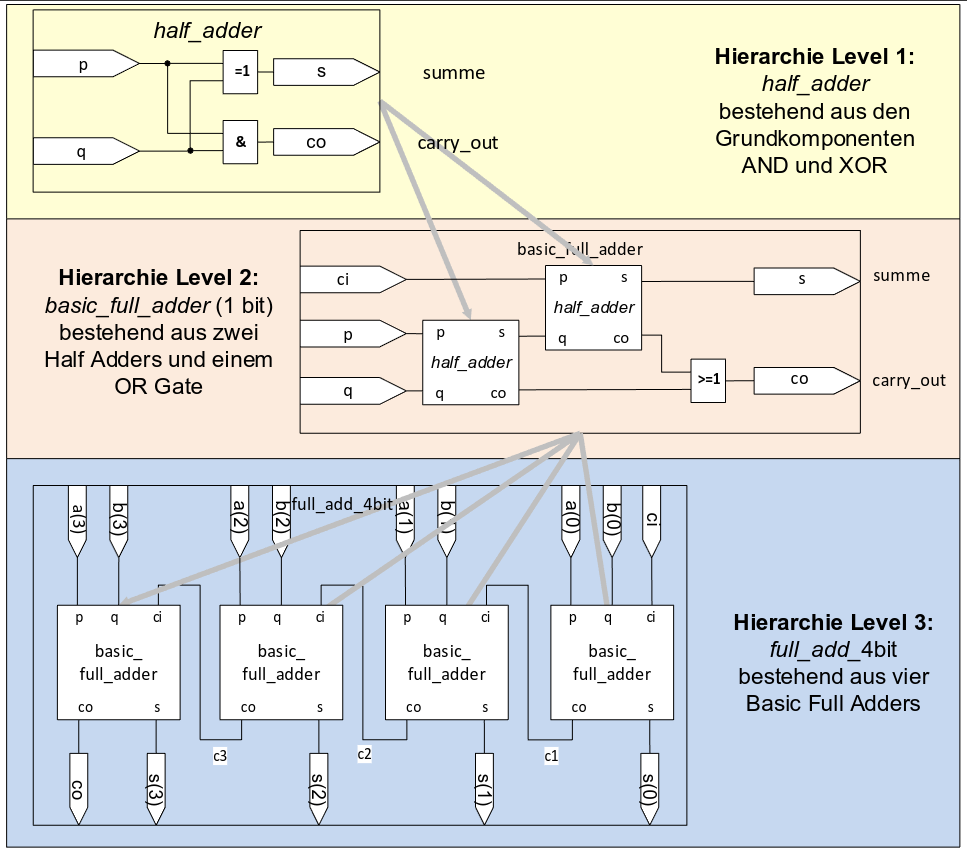
\includegraphics[width=\linewidth]{Images/HierarchienLevel.png}
            \end{minipage}

% ============================================ TIPI =========================================
    \subsection{Tipi}
        \begin{itemize}
            \item \texttt{<architecture\_type>} = \texttt{Behavioral} \textbar{} \texttt{Structural} \textbar{} \texttt{RTL} \textbar{} \texttt{Dataflow} \textbar{} \texttt{Tb} \textbar{} \texttt{(...)} 
            \item \texttt{<mode>} = \texttt{in} \textbar{} \texttt{out} \textbar{} \texttt{inout}
            \item \texttt{<type>} = \texttt{bit} \textbar{} \texttt{bit\_vector} \textbar{} \texttt{std\_}\textcolor{red}{u}\texttt{logic} \textbar{} \texttt{std\_}\textcolor{red}{u}\texttt{logic\_vector} \textbar{} \texttt{integer} \textbar{} \texttt{boolean}
        \end{itemize}
        


% ---------------------------------------- <ARCHITECTURE TYPES> ------------------------------------
        \subsubsection{\texttt{<architecture\_type>}}
            \textbf{Behavioral}: si occupa di descrivere il comportamento del circuito, senza preoccuparsi della struttura fisica. Alto livello di astrazione concetto Wahrheitstabelle.
            \begin{lstlisting}[language=VHDL]
if rising_edge(clk) then
    if A = '1' then
    Y <= B;
    end if;
end if;
            \end{lstlisting}

            \textbf{Structural}: si occupa di descrivere la struttura fisica del circuito, utilizzando componenti e connessioni tra di essi. Medio livello di astrazione.
            \begin{lstlisting}[language=VHDL]
U1: and_gate port map (A => A, B => B, Y => Y1);
U2: or_gate  port map (A =1, B => C, Y => Y);
            \end{lstlisting}

            \textbf{RTL}: si occupa di descrivere il circuito a livello di registro e logica combinatoria, utilizzando registri e porte logiche. Basso livello di astrazione.Concetto Boolsche Ausdrucke.
            \begin{lstlisting}[language=VHDL]
if rising_edge(clk) then
    reg1 <= A and B;
    reg2 <= reg1 xor C;
end if;
            \end{lstlisting}

            \textbf{Dataflow}: si occupa di descrivere il circuito a livello di flusso di dati, utilizzando porte logiche e segnali. Basso livello di astrazione.
            \begin{lstlisting}[language=VHDL]
Y <= (A and B) or (not C);
            \end{lstlisting}

            \textbf{Tb}: si occupa di descrivere il circuito a livello di testbench, utilizzando segnali di test e componenti di test.
            \begin{lstlisting}[language=VHDL]
A <= '0'; wait for 10 ns;
A <= '1'; wait for 10 ns;
assert (Y = expected_value) report "Test failed" severity error;
            \end{lstlisting}

% ---------------------------------------- <TYPES> ------------------------------------
        \subsubsection{\texttt{<type> (dichiarazione: segnali, variabili, ...)}}
        Come vanno dichiarati tutti i segnali utilizzati internamente all'archittetura.\\Nella sintesi del codice, é vietato inizzializzare i segnali nella dichiarazione!
        \begin{itemize}
        \setlength\itemsep{0pt}
            \item \texttt{bit}: rappresenta un singolo bit, con valori \texttt{'0'} e \texttt{'1'}.
            \begin{lstlisting}[language=VHDL]
signal A : bit;
            \end{lstlisting}
            \item \texttt{bit\_vector}: rappresenta un vettore di bit, con valori \texttt{'0'} e \texttt{'1'}.
            \begin{lstlisting}[language=VHDL]
signal B : bit_vector(7 downto 0); -- vettore di 8 bit
            \end{lstlisting}
            \item \texttt{std\_logic}: rappresenta un singolo bit con valori \texttt{'0'}, \texttt{'1'}.
            \begin{lstlisting}[language=VHDL]
signal C : std_logic;
            \end{lstlisting}
            \item \texttt{std\_logic\_vector}: rappresenta un vettore di std\_logic, con valori \texttt{'0'}, \texttt{'1'}.
            \begin{lstlisting}[language=VHDL]
signal D : std_logic_vector(7 downto 0);
            \end{lstlisting}
            \item \texttt{std\_ulogic}: rappresenta un singolo bit con valori \texttt{'0'}, \texttt{'1'}, \texttt{'Z'} (alta impedenza) e \texttt{'X'} (indeterminato).
            \begin{lstlisting}[language=VHDL]
signal E : std_ulogic;
            \end{lstlisting}
            \item \texttt{std\_ulogic\_vector}: rappresenta un vettore di std\_ulogic, con valori \texttt{'0'}, \texttt{'1'}, \texttt{'Z'} e \texttt{'X'}.
            \begin{lstlisting}[language=VHDL]
signal F : std_ulogic_vector(7 downto 0);
            \end{lstlisting}
            \item \texttt{integer}: rappresenta un numero intero, con valori compresi tra $-2^{31}$ e $2^{31}-1$ (è necessario definire l'intervallo di utilizzo).
            \begin{lstlisting}[language=VHDL]
signal G : integer range 0 to 255; -- intervallo di utilizzo
            \end{lstlisting}
            \item \texttt{boolean}: rappresenta un valore booleano, con valori \texttt{true} e \texttt{false}.
            \begin{lstlisting}[language=VHDL]
signal H : boolean; -- true or false
            \end{lstlisting}
        \end{itemize}
        
% ============================================ PARALLEL SIGNAL =========================================
    \subsection{Nebenläufige Signalzuweisungen "y<=x"}
        \subsubsection{Definizione dei segnali}
            \begin{lstlisting}[language=VHDL]
singal <signal_name> :{,<singal_name>} : <type>
[:= inizianol_value]; -- inizial_value é opzionale
            \end{lstlisting}
    
    % ------------------------------ UNCONDITIONAL -----------------
        \subsubsection{Unbedingte Signalzuweisung}
            L'assegnazione dei segnali é incondizionata, quindi indipendente.
            \begin{lstlisting}[language=VHDL]
y <= '0';
y <= a and b;
            \end{lstlisting}
    
    % ------------------------------ CONDITIONAL -----------------
        \subsubsection{Bedingte Signalzuweisung}
            L'assegnazione dei segnali é eseguita in modo sequenziale, si controlla una condizione e se corretta si assegna il valore, sennó si procede con la prossima condizione.
            \begin{lstlisting}[language=VHDL]
y <= '0' when a = '1' else 
        '1' when a = '0';
            \end{lstlisting}
    
    % ------------------------------ SELECTIVE -----------------
        \subsubsection{Selektive Signalzuweisung}
            L'assegnazione dei segnali é eseguita in modo selettivo, viene selezionata il valore in base alla condizione.
            \begin{lstlisting}[language=VHDL]
with s select y <=
    '0' when "00", -- quando s = "00" y <= '0'
    '1' when "01", -- quando s = "01" y <= '1'
    'Z' when "10", -- quando s = "10" y <= 'Z'
    'X' when others; -- quando s =  altro y <= 'X'
            \end{lstlisting}
    
    % ------------------------------ AGGREGATE -----------------
        \subsubsection{aggregate}
            L'aggregazione dei segnali permette di aggregare segnali individuali in un unico segnale.
            \begin{lstlisting}[language=VHDL]
y <= (a, b, '1', '0'); -- Assegnazione implicita
y <= (0 => '0', 1 => '1', 2 => b, others => a); -- Assegnazione esplicita (<posizione_vettoriale> => <valore>)
            \end{lstlisting}
    
    % ------------------------------ CONCATENATE -----------------
        \subsubsection{concatenate}
            La concatenazione dei segnali permette di concatenare segnali in un unico segnale.
            \begin{lstlisting}[language=VHDL]
y <= v_1 & v_2;
            \end{lstlisting}


% ========================================= PROCESSI =========================================
    \subsection{Nebenläufige Prozesse}
        I processi sono "Nebenläufige" di conseguenza iniziano ad essere eseguiti in concorrenza. Ma all'interno il codice viene eseguito normalmente (istruzioni sequenziali, sequenzialmente. istruzioni parallele in modo parallelo).\\
        I processi sono sezioni di codice che vengono eseguite ogni volta che un \textcolor{red}{Segnale sensibile} nella lista sensibile (Sensitivitätliste) cambia di stato.         % Inizia un codice blocco, con colori VHDL (vedi definizione in DigDes.tex), escape inside is used to use external commandstf
        \begin{lstlisting}[language=VHDL, escapeinside={(*@}{@*)}, numberstyle=\tiny\color{gray}\highlightlines{3,4,5,6,7}{green}]
process ((*@\textcolor{red}{clk, reset}@*))
    begin
        if reset = '1' then
            -- inserisci il codice da eseguire in caso di reset
        elsif rising_edge(clk) then
            -- inserisci il codice da eseguire ad ogni fronte di salita del clock
        end if;
    end process;
        \end{lstlisting}
    
    % ------------------------------ SEQUENZIELLE ANWEISUNGEN IM PROZESSE -----------------
        \subsubsection{sequenzielle Anweisungen im Prozesse}
            Le istruzioni che vengono eseguite strettamente sequenzialmente all'interno di un processo sono:
            \begin{lstlisting}[language=VHDL]
-- struttura if else:
if condition_a then
    {sequential statements}
elsif condition_b then
    {sequential statements}
else
    {sequential statements}
end if;


-- struttura case when:
case expression is
    when choice_a => {sequential statements}
    when choice_b => {sequential statements}
    when others => {sequential statements}
end case;
            \end{lstlisting}
    
    % ------------------------------ Eigenschaften nebenläufiger Prozesse -----------------
        \subsubsection{Eigenschaften nebenläufiger Prozesse}
        Le proprietà più importanti, ovvero le estensioni rispetto alle assegnazioni di segnale, possono essere così riassunte:
            \begin{itemize}
                \item I processi possono assegnare due o più segnali contemporaneamente.
                \item L'elaborazione delle informazioni per l'assegnazione dei segnali avviene in una sequenza di comandi che vengono eseguiti uno dopo l'altro (procedurale).
                \item I processi permettono l'uso di variabili per la memorizzazione temporanea dei valori dei segnali.
                \item Grazie all'uso delle liste di sensibilità è garantito un miglior controllo sulle condizioni di esecuzione della parte di codice.
            \end{itemize}
    
    % ------------------------------ Variablen in nebenläufigen Prozessen -----------------
        \subsubsection{Variablen in nebenläufigen Prozessen}
        Le variabili offrono due opzioni utili nei processi:
            \begin{itemize}
                \item Accesso a un valore aggiornato all'interno del processo stesso.
                \item Preparazione di un'espressione di controllo, ad esempio per un "case when".
            \end{itemize}
            Le variabili sono dichiarate all'interno dei processi e sono visibili esclusivamente all'interno degli stessi.
            Il valore assegnato può essere letto immediatamente.\\
            L'assegnazione di valore a una variabile avviene con l'operatore :=, a differenza dell'assegnazione ai segnali che utilizza <=.
        \begin{lstlisting}[language=VHDL]
variable <var_name> {,var_name}: <type> [:= expression];
        \end{lstlisting}
        \section{State machine}
    Le \textbf{Finite State Machine} (FSM) sono circuiti sequenziali che possono essere in uno stato tra un insieme finito di stati. 
    La transizione tra gli stati avviene in base a segnali di ingresso e può essere condizionata da segnali di clock e reset.

    \begin{minipage}[t]{1\columnwidth}
        \vspace{0pt} % <-- ensures top alignment
        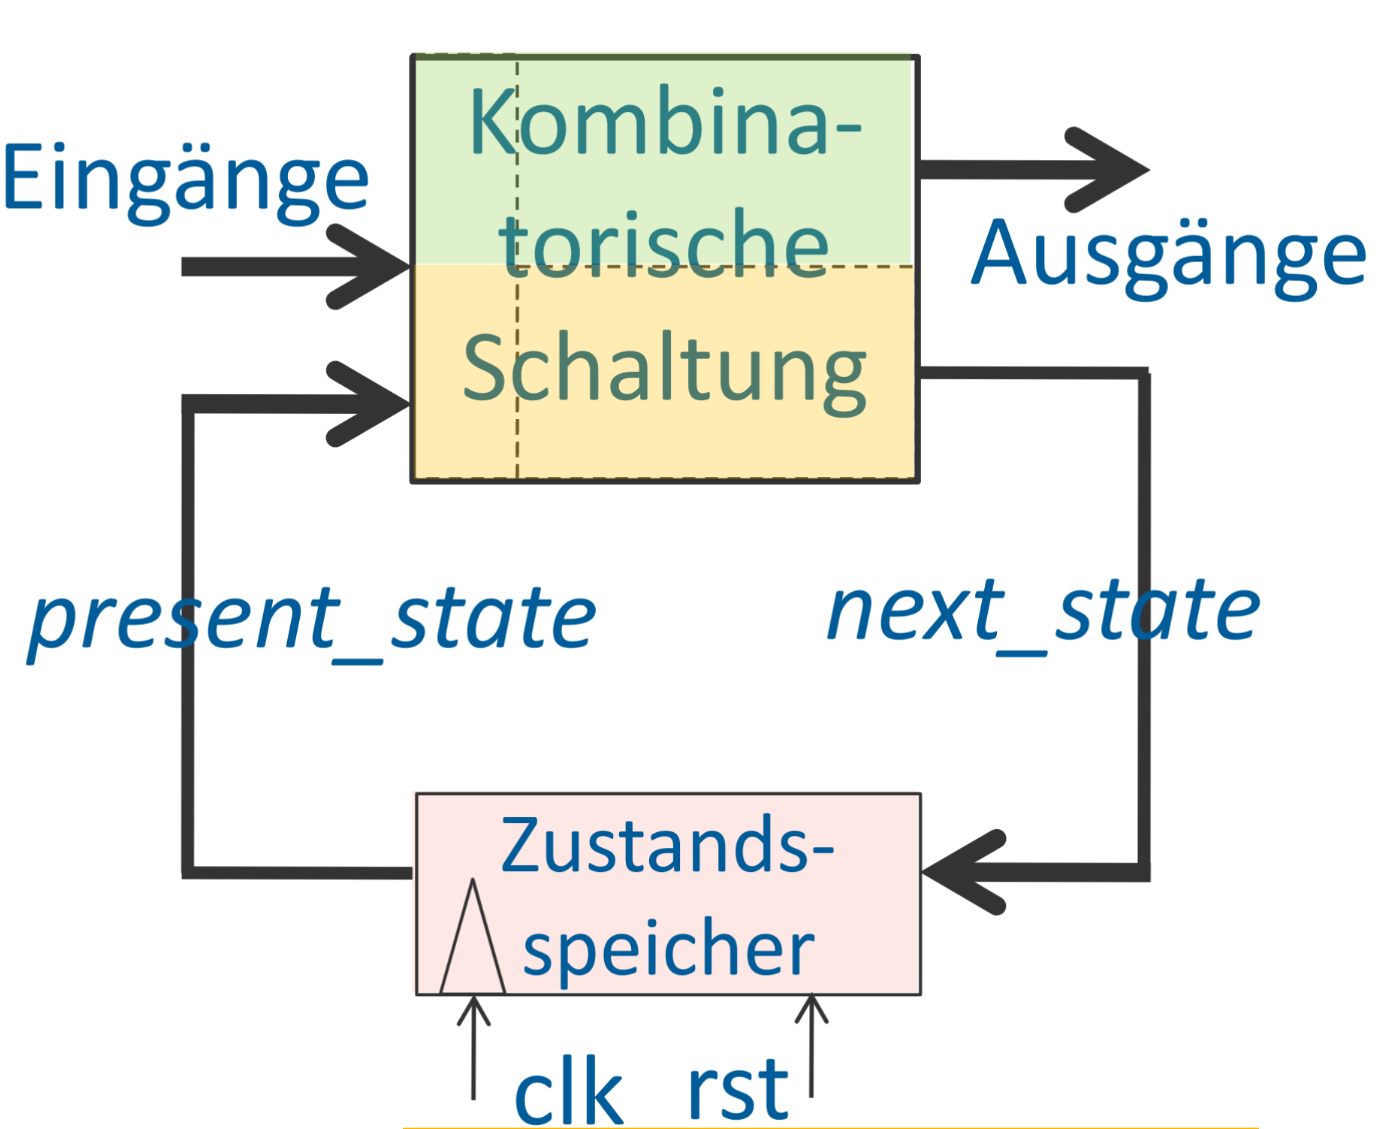
\includegraphics[width=\linewidth]{Images/FSMGeneralizzata.png}
    \end{minipage}%
    

% ==================================== CODICE SCHELETRO FSM ====================================
    \subsection{Codice scheletro FSM (f,g,z)}


% ==================================== CODIFICA DEGLI STATI ====================================
    \subsection{Codifica degli stati}
    Gli stati di una FSM possono essere codificati in diversi modi, tra cui:
    \begin{itemize}
        \item \textbf{Codifica binaria}: ogni stato è rappresentato da un codice binario unico.
        \item \textbf{Codifica Gray}: simile alla codifica binaria, ma le transizioni tra stati adiacenti cambiano solo un bit alla volta.
        \item \textbf{Codifica one-hot}: ogni stato è rappresentato da un bit attivo, con tutti gli altri bit a zero.
        \item \textbf{Codifica one-cold}: simile alla codifica one-hot, ma solo un bit è a zero e tutti gli altri sono attivi.
    \end{itemize}
        \section{Sostituzione discreta per segnali elettrici}


% ==================================== ELETRIC SIGNALS ====================================
\subsection{Segnali elettrici}

\begin{center}
    \begin{adjustbox}{max width=\columnwidth}
        \begin{tabular}{|l|l|p{6cm}|c|}
            \hline
            \multicolumn{1}{|c|}{\shortstack{\textbf{Logik}\\\textbf{-wert}}} & 
            \multicolumn{1}{c|}{\textbf{Bedeutung}} & 
            \multicolumn{1}{c|}{\textbf{Verwendung}} & 
            \multicolumn{1}{c|}{\shortstack{\textbf{Für Logik}\\\textbf{Synthese}}} \\
                \hline
                \verb|'U'| & Uninitialized   & Signal ist im Simulator noch nicht initialisiert. In der Hardware ist das Signal unbekannt. Typisch für nicht initialisierte Speicherstelle nach Start-up. & Nein \\
                \hline
                \verb|'X'| & Undefined       & Signal ist dem Simulator unbekannt. Typisch für Treiberkonflikte, d.h. ein Signal wird von mehr als einer Quelle getrieben. In der Welt der Hardware kommt dies vor allem bei Buskonflikten vor. & Nein \\
                \hline
                \verb|'0'| & Strong zero     & Low Pegel eines Standardausganges. Regelfall für Hardware „0“ Pegel. & Ja \\
                \hline
                \verb|'1'| & Strong one      & High Pegel eines Standardausganges. Regelfall für Hardware „1“ Pegel. & Ja \\
                \hline
                \verb|'Z'| & High Impedance  & Signalausgang von Leitung entkoppelt. Typisch für Hochimpedanz Ausgang eines Three-State Treibers bei bidirektionalen Bussen. & Ja \\
                \hline
                \verb|'L'| & Weak zero       & Low Pegel eines schwachen Treiberausgangs. Typisch für ein Signal, das mit einem pull-down Widerstand auf Low Potenzial gezogen wird. & Nein \\
                \hline
                \verb|'H'| & Weak one        & High Pegel eines schwachen Treiberausgangs. Typisch für ein Signal, das mit einem pull-up Widerstand auf High Potenzial gezogen wird. & Nein \\
                \hline
                \verb|'W'| & Weak unknown    & Simulator erkennt Treiberkonflikt. Dieser Fall ist analog zu \verb|'X'| mit dem Unterschied, dass der Treiberkonflikt hier durch schwache Treiber verursacht wird. & Nein \\
                \hline
                \verb|'-'| & Don’t Care      & Logikzustand des Ausgangssignals ist bedeutungslos. Existiert nur in der Schaltungssynthese und wird für Logikminimierung gebraucht. & Nein \\
                \hline
        \end{tabular}
    \end{adjustbox}
\end{center}
        \section{Examples}
% ==================== FILP FLOP ========================
    \subsection{Flip flop}
    \begin{lstlisting}[language=VHDL, escapeinside={(*@}{@*)}]
entity d_ff_rst is
    port(
        clk : in bit;
        rst : in bit;
        d : in bit;
        q : out bit
        );
end d_ff_rst;
    
architecture behavioral of d_ff_rst is
begin
    register : process(clk, rst)
            -- d fehlt in Sens.list
    begin   -- Nur clk und Reset
            -- aktivieren Prozess
        if (rst = '1') then
            -- Asynchroner Reset
            q <= '0';
            -- wird zuerst abgearbeitet
        elsif (clk(*@'@*)event and clk = '1') then (*@\setlength{\fboxsep}{1pt}\colorbox{yellow}{\strut\textbf{\textcolor[rgb]{0.0,0.4,0.2}{-- Sintassi per la detezione del fianco salita del clock}}}@*)
            q <= d; -- Synchroner Teil
        end if; -- Kein abschliessendes
        -- else: in allen anderen
    end process; -- Fällen wird gespeichert.
end behavioral;
    \end{lstlisting}
        \section{notebooklm.tex}

\textbf{\texttt{std\_ulogic} (unresolved)} [8]:
\begin{itemize}
    \item Replaces \texttt{bit} type [8].
    \item \textbf{Allows only one driver per signal}; compiler reports error on multiple drivers [8].
    \item Suitable for three-state outputs using 'Z' [9].
    \item Recognises uninitialized ('U'), weak ('H', 'L'), and don't care ('-') states [9, 10].
    \item Recommended for educational projects for its strictness [11].
\end{itemize}

\textbf{\texttt{std\_logic} (resolved)} [10]:
\begin{itemize}
    \item Removes the 'unresolved' restriction, allowing multiple drivers [10].
    \item \textbf{Simulator automatically resolves driver conflicts} based on a resolution function (e.g., '0' and '1' resolving to 'X', '0' and 'Z' to '0') [10, 12].
    \item More prone to hidden errors (compiler won't catch multiple assignments) [13].
    \item Widely used in practice for its flexibility, especially for physical implementation concerns [14].
    \item In VHDL 2008, \texttt{std\_logic} is a subtype of \texttt{std\_ulogic} [15].
\end{itemize}
\subsubsection{Modelling Bidirectional Buses in VHDL}
\begin{itemize}[leftmargin=1.5em]
    \item Uses the \textbf{\texttt{inout}} port mode.
    \item Writing to the bus: \verb|bus_i_o <= out_i when enable = '1' else (others => 'Z');|
    \item Reading from the bus: \verb|in_i <= bus_i_o;|
\end{itemize}

\subsection{VHDL Key Concept IV: Event-Based Concept for Temporal Representation in Simulations}

\subsubsection{Simulation as a Central Step}
\begin{itemize}[leftmargin=1.5em]
    \item Crucial for design verification.
    \item \textbf{Reusable Test-Benches} help with regression testing.
    \item \textbf{Later error detection is more costly.}
\end{itemize}

\subsubsection{Modelling Temporal Behaviour}
\begin{itemize}[leftmargin=1.5em]
    \item \textbf{Event Queue:} Simulators use an event queue to process events in order.
    \item \textbf{Delta-Time Model:}
    \begin{itemize}
        \item Functional simulation model.
        \item Infinitesimal time delay (\textit{delta cycle}).
        \item Ensures cause-effect separation in waveform views.
    \end{itemize}
    \item \textbf{Transport Delay:}
    \begin{itemize}
        \item Models real delay.
        \item Syntax: \verb|B <= transport A after tp;|
        \item \textbf{All pulses propagate}.
    \end{itemize}
    \item \textbf{Inertial Delay (default):}
    \begin{itemize}
        \item Models physical filtering of glitches.
        \item Syntax: \verb|B <= A after tp;|
        \item \textbf{Short pulses filtered out}.
    \end{itemize}
\end{itemize}

\subsubsection{Simulation Setup (Test-Bench)}
\begin{itemize}[leftmargin=1.5em]
    \item Not synthesizable.
    \item \textbf{Device Under Test (DUT)}: Component under test.
    \item \textbf{Stimulus Generator}: Drives input signals.
    \item \textbf{Response Monitor}: Verifies DUT output.
    \item \textbf{\texttt{ASSERT}} Statement:
    \begin{itemize}
        \item Syntax: \verb|assert (cond) report "msg" severity level;|
        \item Levels: \texttt{note}, \texttt{warning}, \texttt{error}, \texttt{failure}.
    \end{itemize}
\end{itemize}

\subsection{VHDL Key Concept VIII: Arithmetic and Data Types}

\subsubsection{Arithmetic Operations}
\begin{itemize}[leftmargin=1.5em]
    \item Problem: \texttt{bit\_vector}, \texttt{std\_logic\_vector} don't support arithmetic.
    \item Solution: Use \texttt{ieee.numeric\_std}.
    \item Defines:
    \begin{itemize}
        \item \textbf{\texttt{signed}}: For signed numbers.
        \item \textbf{\texttt{unsigned}}: For unsigned numbers.
    \end{itemize}
    \item Functions: \texttt{+}, \texttt{-}, \texttt{}, \texttt{abs}, \texttt{/}, \texttt{mod}, \texttt{rem}, \texttt{**} (limited).
    \item Prefer \texttt{numeric\_std} over older \texttt{std\_logic\_signed} or \texttt{unsigned}.
\end{itemize}

\subsubsection{Data Types}
\begin{itemize}[leftmargin=1.5em]
    \item Strong typing enforces correctness.
    \item \textbf{Scalar Types:}
    \begin{itemize}
        \item Discrete: \texttt{integer}, \texttt{boolean}, \texttt{bit}, \texttt{std\_ulogic}, etc.
        \item Physical: \texttt{time}, etc.
    \end{itemize}
    \item \textbf{Composite Types:}
    \begin{itemize}
        \item Arrays: \texttt{std\_logic\_vector}, etc.
        \item Records: Heterogeneous collections.
    \end{itemize}
\end{itemize}

\subsubsection{Type Conversion}
\begin{itemize}[leftmargin=1.5em]
    \item \textbf{\texttt{resize}}: For \texttt{signed}/\texttt{unsigned} vectors.
    \item \textbf{Type Casting:}
    \begin{itemize}
        \item Syntax: \verb|target_type(signal)|
        \item Example: \verb|o_int <= unsigned(a) + unsigned(b);|
    \end{itemize}
    \item \textbf{Type Conversion Functions:}
    \begin{itemize}
        \item Between different base types.
        \item Examples: \verb|to_unsigned(int, len)|, \verb|to_integer(vec)|
    \end{itemize}
\end{itemize}

\subsection{VHDL Key Concept IX: Parametrisability of Models}

\subsubsection{Reusability}
\begin{itemize}[leftmargin=1.5em]
    \item \textbf{Essential for efficient design}.
    \item General models can be adapted via parameters.
\end{itemize}

\subsubsection{Using \texttt{generic}}
\begin{itemize}[leftmargin=1.5em]
    \item Allows time-invariant parameters in \texttt{entity}.
    \item Example: \verb|generic(max_count: integer := 127);|
    \item Used for widths, delays, strengths.
    \item Assigned via \texttt{generic map}:
    \begin{itemize}
        \item \verb|instance_name : component_name generic map (...) port map (...);|
    \end{itemize}
\end{itemize}

\subsubsection{Timing of Parameter Fixation}
\begin{itemize}[leftmargin=1.5em]
    \item \textbf{Design-time}: via \texttt{constant}.
    \item \textbf{Compile-time}: via \texttt{generic}.
    \item \textbf{Runtime}: via \texttt{signal} assignments.
\end{itemize}

    \end{multicols}
\end{document}

% TODO:
% aggiungiere comando per le linee colorate in modo che posso colorarne diverse con colori diversi (cheatsheettemplate)
% aggiungere al comando titolo animegirl ganbatteneeee!! (cheatsheettemplate)
% aggiungere al comando titolo collaboartori